\documentclass[tikz]{standalone}


\usetikzlibrary{shapes, shapes.geometric, shapes.misc, shapes.arrows}
\usetikzlibrary{angles, math, calc, matrix}
\usetikzlibrary{circuits.ee.IEC}
% This bascially automates a \newcommand{<name>}{} to ensure
% that a command with the given <name> does not already exist
\providecommand*{\pgfmathsetnewmacro}[2]{%
    \newcommand*{#1}{}% Error if already defined
    \pgfmathsetmacro{#1}{#2}%
}%

\begin{document}
    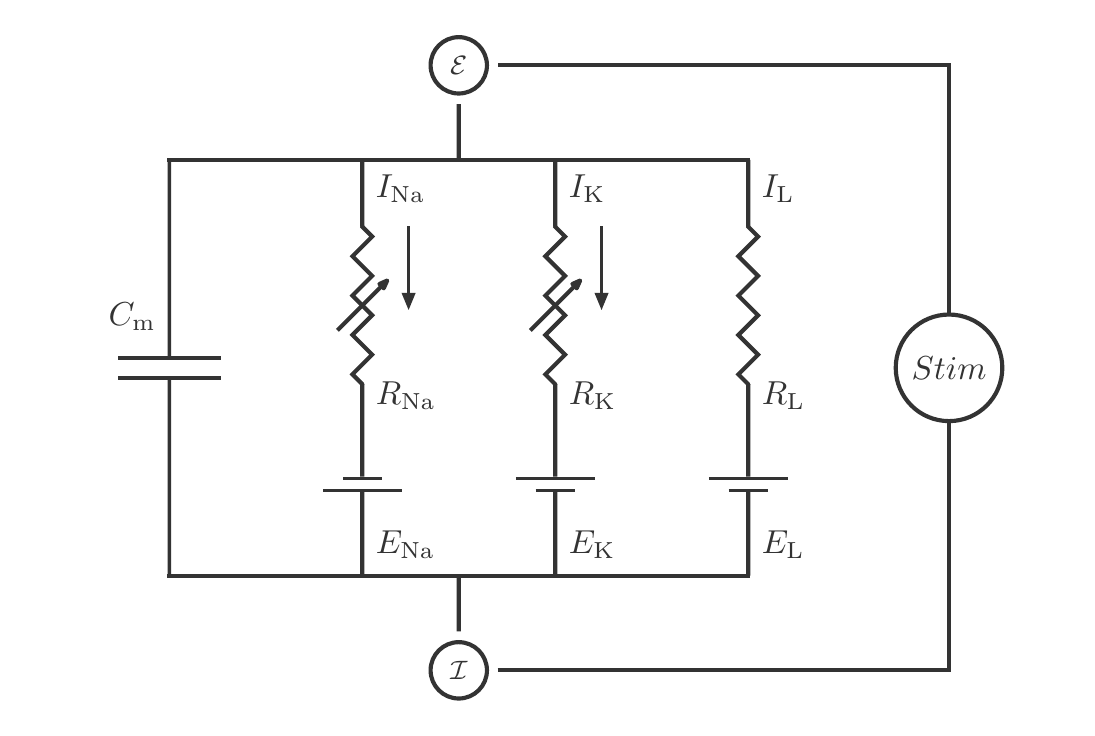
\begin{tikzpicture}[
    %x=1cm, y=1cm, 
    %z={(0cm,1cm)},
    scale = 1.2,
    transform shape,
    line width = 1.5pt, 
    black!80,
    circuit ee IEC,
    every info/.style={font=\footnotesize},
        small circuit symbols,
            set resistor graphic=var resistor IEC graphic,
            set diode graphic=var diode IEC graphic,
            set make contact graphic= var make contact IEC graphic
    ]

    % Determines the boundries
    \path[use as bounding box] (-4.5,-3.6) rectangle (6.5,3.6);

    \pgfmathsetnewmacro\circuitR{0.5}             % radius of heads
    \pgfmathsetnewmacro\circuitS{0.5}             % scale
    \pgfmathsetnewmacro\circuitL{2}               % length
    \pgfmathsetnewmacro\circuitW{0.75}            % width
    \pgfmathsetnewmacro\circuitWl{1}              % width of the lipids
    \pgfmathsetnewmacro\circuitWc{1.30}           % width of the capacitor
    \pgfmathsetnewmacro\circuitJ{2cm}             % not too sure
    \pgfmathsetnewmacro\chanGap{3cm}
    \pgfmathsetnewmacro\exShift{3}
    \pgfmathsetnewmacro\circuitSteps{4}

    % Ratio for each ion
    \pgfmathsetnewmacro\Capr{1/10}
    \pgfmathsetnewmacro\Lr{11/12}
    \pgfmathsetnewmacro\Curr{12/10}
    \pgfmathsetnewmacro\Nar{1/3}
    \pgfmathsetnewmacro\Kr{2/3}
    % \pgfmathsetnewmacro\Nas{Na}
    %\pgfmathsetnewmacro\Kr{3/12}
    %\pgfmathsetnewmacro\Nar{7/12}
    %\pgfmathsetnewmacro\Nar{1/(2*\circuitR*\circuitS)}
    \pgfmathsetnewmacro\Clr{11/12}

    % Definining the coordinates of the box corners
    \pgfmathsetnewmacro\boxRise{2.2}
    \pgfmathsetnewmacro\boxRun{3.75}
    
    \coordinate (O)  at (0,0);
    \coordinate (TR) at ( \boxRun, \boxRise);
    \coordinate (TL) at (-\boxRun, \boxRise);
    \coordinate (BL) at (-\boxRun,-\boxRise);
    \coordinate (BR) at ( \boxRun,-\boxRise);

    % Define centers of the walls of the circuit
    \coordinate (CC) at ($($(TL)!\Capr!(TR)$)!1/2!($(BL)!\Capr!(BR)$)$);
    \coordinate (LC) at ($($(TL)!\Lr!(TR)$)!1/2!($(BL)!\Lr!(BR)$)$);
    
    % Define centers of the floor and ceiling of the circuit
    \coordinate (EM) at ($($(TL)!\Capr!(TR)$)!1/2!($(TL)!\Lr!(TR)$)$);
    \coordinate (IM) at ($($(BL)!\Capr!(BR)$)!1/2!($(BL)!\Lr!(BR)$)$);

    
    % Underlines Circuit
    \begin{scope}[white, line width = 5pt]
    % Leakage
        \draw ($(TL)!\Lr!(TR)$) to [resistor={pos = 0.40}, 
            battery={pos = 0.70, minimum height=0.75cm, minimum width=0.15cm, line cap = rect}
            ]%
            node [pos = 0.5, anchor = north west, xshift = -3.5]{$R_\mathrm{L}$}%
            ($(BL)!\Lr!(BR)$);
              
        % Underlines circuit
        \draw[line cap = rect] ($(TL)!\Capr!(TR)$) -- ($(TL)!\Lr!(TR)$) 
                               ($(BL)!\Capr!(BR)$) -- ($(BL)!\Lr!(BR)$);
    \end{scope}
        
    \begin{scope}[line width = 1.5pt] % Draws the visible circuit
        % Marks the extternal Nodes
        \path (EM)+( 90: 1) node (E) [circle, minimum width = 0.77cm, fill = white]{};
        \path (IM)+(-90: 1) node (I) [circle, minimum width = 0.77cm, fill = white]{};
    
        % Underlines Node to Cicuit
        \draw[white, line width = 5pt] 
              (E) to (EM)
              (I) to (IM);
              
        % Overlines Node to Cicuit
        \draw (E) to (EM)
              (I) to (IM);

         % Nodes
        \node at (I) [circle,draw, fill = white] {\footnotesize $\mathcal{I}$};
        \node at (E) [circle,draw, fill = white] {\footnotesize $\mathcal{E}$};
        
        % Overlines circuit
        \draw[line cap = rect] ($(TL)!\Capr!(TR)$) -- ($(TL)!\Lr!(TR)$) 
                               ($(BL)!\Capr!(BR)$) -- ($(BL)!\Lr!(BR)$);


        % Internal labeling and circutry
        \begin{scope}[align=left]
        \foreach \F/\I/\R/\A in 
            {\Nar/Na/0/adjustable', \Kr/K/180/adjustable', 1/L/180/}{
            % Making the main circuit paths
            \draw%
            ($($(BL)!\Capr!(BR)$)!\F!($(BL)!\Lr!(BR)$)$) to%
            [battery={pos = 0.22, minimum height=1cm, minimum width=0.15cm, rotate = \R, line width = 1.2pt},% 
            resistor={\A, pos = 0.65, minimum height=0.25cm, minimum width = 2cm}]%
            node[pos = 0.5, anchor = north west, xshift = 0]%
            {$R_\mathrm{\I}$}%
            ($($(TL)!\Capr!(TR)$)!\F!($(TL)!\Lr!(TR)$)$);
    
            % Making external markings
            \path%
            ($($(TL)!\Capr!(TR)$)!\F!($(TL)!\Lr!(TR)$)$) -- % 
            ($($(BL)!\Capr!(BR)$)!\F!($(BL)!\Lr!(BR)$)$) node (I\I) 
                [pos = 0.069, anchor = west]  
                {$I_{\mathrm{\I}}$};
            
            \path%
            ($($(TL)!\Capr!(TR)$)!\F!($(TL)!\Lr!(TR)$)$) -- % 
            ($($(BL)!\Capr!(BR)$)!\F!($(BL)!\Lr!(BR)$)$) node (E\I) 
                [pos = 0.925, anchor = west]  
                {$E_{\mathrm{\I}}$};
    
            \foreach \o in {-,+}{%
                \path% 
                ($($(TL)!\Capr!(TR)$)!\F!($(TL)!\Lr!(TR)$)$) -- % 
                ($($(BL)!\Capr!(BR)$)!\F!($(BL)!\Lr!(BR)$)$) 
                    node (S\I\o) [pos = 0.70, anchor = east, inner sep=0pt, xshift = -0.35cm, yshift = \o 0.28 cm] {};
            }
        }

        \draw%
            (I) -| ($(BL)!\Curr!(BR)$) to%
            node[midway, draw, fill = white, circle] {$Stim$}%
            ($(TL)!\Curr!(TR)$) |- (E);
    
        % Arrows
        \foreach \ind in {\Kr, \Nar}{% 
            \draw[line width = 1pt]%
            ($($(TL)!\Capr!(TR)$)!\ind+0.08!($(TL)!\Lr!(TR)$)$)++(0,-0.70cm)%
            -- ++(0,-0.75cm) 
            node[isosceles triangle, scale = 0.25, draw, fill, rotate = 270] {};
        }

        % Arrowing each side
        \path ($(BL)!\Nar!(BR)$) -- +(0, 0.25) coordinate (BE)
              ($(TL)!\Nar!(TR)$) -- +(0,-0.25) coordinate (TE);
        \end{scope}
        
        % Capacitance shit
        \draw[line cap = rect, line width = 1.2pt]%
            ($(BL)!\Capr!(BR)$) to%
            [capacitor={minimum height= \circuitWc cm, minimum width = 0.25 cm}]%
            ($(TL)!\Capr!(TR)$);
        \path%
            ($(BL)!\Capr!(BR)$) -- ($(TL)!\Capr!(TR)$)%
            node[midway, anchor = south east, yshift = 0.25cm] {$C_\mathrm{m}$};

        \path (CC)++( 90:\circuitL * \circuitS +  \circuitR * \circuitS  + \exShift * \circuitS  cm) -- +(0:0.5*\circuitWc) coordinate (PR) -- +(180:0.5*\circuitWc) coordinate (PL);
        \path (CC)++(-90:\circuitL * \circuitS +  \circuitR * \circuitS  + \exShift * \circuitS  cm) -- +(0:0.5*\circuitWc) coordinate (NR) -- +(180:0.5*\circuitWc) coordinate (NL);
    \end{scope}
    \end{tikzpicture}
\end{document}